%
% The Computer Society usually requires 12pt for submissions.
%
\documentclass[12pt,journal,compsoc]{IEEEtran}
%
% If IEEEtran.cls has not been installed into the LaTeX system files,
% manually specify the path to it like:
% \documentclass[12pt,journal,compsoc]{../sty/IEEEtran}

\usepackage{amsmath}
\usepackage{graphicx}

\usepackage[hidelinks]{hyperref}

\usepackage{amsfonts}

\usepackage[utf8]{inputenc} 
\usepackage[ngerman]{babel} 

% Some very useful LaTeX packages include:
% (uncomment the ones you want to load)


% *** MISC UTILITY PACKAGES ***
%
%\usepackage{ifpdf}
% Heiko Oberdiek's ifpdf.sty is very useful if you need conditional
% compilation based on whether the output is pdf or dvi.
% usage:
% \ifpdf
%   % pdf code
% \else
%   % dvi code
% \fi
% The latest version of ifpdf.sty can be obtained from:
% http://www.ctan.org/tex-archive/macros/latex/contrib/oberdiek/
% Also, note that IEEEtran.cls V1.7 and later provides a builtin
% \ifCLASSINFOpdf conditional that works the same way.
% When switching from latex to pdflatex and vice-versa, the compiler may
% have to be run twice to clear warning/error messages.






% *** CITATION PACKAGES ***
%
\ifCLASSOPTIONcompsoc
  % IEEE Computer Society needs nocompress option
  % requires cite.sty v4.0 or later (November 2003)
  % \usepackage[nocompress]{cite}
\else
  % normal IEEE
  % \usepackage{cite}
\fi
% cite.sty was written by Donald Arseneau
% V1.6 and later of IEEEtran pre-defines the format of the cite.sty package
% \cite{} output to follow that of IEEE. Loading the cite package will
% result in citation numbers being automatically sorted and properly
% "compressed/ranged". e.g., [1], [9], [2], [7], [5], [6] without using
% cite.sty will become [1], [2], [5]--[7], [9] using cite.sty. cite.sty's
% \cite will automatically add leading space, if needed. Use cite.sty's
% noadjust option (cite.sty V3.8 and later) if you want to turn this off.
% cite.sty is already installed on most LaTeX systems. Be sure and use
% version 4.0 (2003-05-27) and later if using hyperref.sty. cite.sty does
% not currently provide for hyperlinked citations.
% The latest version can be obtained at:
% http://www.ctan.org/tex-archive/macros/latex/contrib/cite/
% The documentation is contained in the cite.sty file itself.
%
% Note that some packages require special options to format as the Computer
% Society requires. In particular, Computer Society  papers do not use
% compressed citation ranges as is done in typical IEEE papers
% (e.g., [1]-[4]). Instead, they list every citation separately in order
% (e.g., [1], [2], [3], [4]). To get the latter we need to load the cite
% package with the nocompress option which is supported by cite.sty v4.0
% and later. Note also the use of a CLASSOPTION conditional provided by
% IEEEtran.cls V1.7 and later.





% *** GRAPHICS RELATED PACKAGES ***
%
\ifCLASSINFOpdf
  % \usepackage[pdftex]{graphicx}
  % declare the path(s) where your graphic files are
  % \graphicspath{{../pdf/}{../jpeg/}}
  % and their extensions so you won't have to specify these with
  % every instance of \includegraphics
  % \DeclareGraphicsExtensions{.pdf,.jpeg,.png}
\else
  % or other class option (dvipsone, dvipdf, if not using dvips). graphicx
  % will default to the driver specified in the system graphics.cfg if no
  % driver is specified.
  % \usepackage[dvips]{graphicx}
  % declare the path(s) where your graphic files are
  % \graphicspath{{../eps/}}
  % and their extensions so you won't have to specify these with
  % every instance of \includegraphics
  % \DeclareGraphicsExtensions{.eps}
\fi
% graphicx was written by David Carlisle and Sebastian Rahtz. It is
% required if you want graphics, photos, etc. graphicx.sty is already
% installed on most LaTeX systems. The latest version and documentation can
% be obtained at: 
% http://www.ctan.org/tex-archive/macros/latex/required/graphics/
% Another good source of documentation is "Using Imported Graphics in
% LaTeX2e" by Keith Reckdahl which can be found as epslatex.ps or
% epslatex.pdf at: http://www.ctan.org/tex-archive/info/
%
% latex, and pdflatex in dvi mode, support graphics in encapsulated
% postscript (.eps) format. pdflatex in pdf mode supports graphics
% in .pdf, .jpeg, .png and .mps (metapost) formats. Users should ensure
% that all non-photo figures use a vector format (.eps, .pdf, .mps) and
% not a bitmapped formats (.jpeg, .png). IEEE frowns on bitmapped formats
% which can result in "jaggedy"/blurry rendering of lines and letters as
% well as large increases in file sizes.
%
% You can find documentation about the pdfTeX application at:
% http://www.tug.org/applications/pdftex





% *** MATH PACKAGES ***
%
%\usepackage[cmex10]{amsmath}
% A popular package from the American Mathematical Society that provides
% many useful and powerful commands for dealing with mathematics. If using
% it, be sure to load this package with the cmex10 option to ensure that
% only type 1 fonts will utilized at all point sizes. Without this option,
% it is possible that some math symbols, particularly those within
% footnotes, will be rendered in bitmap form which will result in a
% document that can not be IEEE Xplore compliant!
%
% Also, note that the amsmath package sets \interdisplaylinepenalty to 10000
% thus preventing page breaks from occurring within multiline equations. Use:
%\interdisplaylinepenalty=2500
% after loading amsmath to restore such page breaks as IEEEtran.cls normally
% does. amsmath.sty is already installed on most LaTeX systems. The latest
% version and documentation can be obtained at:
% http://www.ctan.org/tex-archive/macros/latex/required/amslatex/math/





% *** SPECIALIZED LIST PACKAGES ***
%
%\usepackage{algorithmic}
% algorithmic.sty was written by Peter Williams and Rogerio Brito.
% This package provides an algorithmic environment fo describing algorithms.
% You can use the algorithmic environment in-text or within a figure
% environment to provide for a floating algorithm. Do NOT use the algorithm
% floating environment provided by algorithm.sty (by the same authors) or
% algorithm2e.sty (by Christophe Fiorio) as IEEE does not use dedicated
% algorithm float types and packages that provide these will not provide
% correct IEEE style captions. The latest version and documentation of
% algorithmic.sty can be obtained at:
% http://www.ctan.org/tex-archive/macros/latex/contrib/algorithms/
% There is also a support site at:
% http://algorithms.berlios.de/index.html
% Also of interest may be the (relatively newer and more customizable)
% algorithmicx.sty package by Szasz Janos:
% http://www.ctan.org/tex-archive/macros/latex/contrib/algorithmicx/




% *** ALIGNMENT PACKAGES ***
%
%\usepackage{array}
% Frank Mittelbach's and David Carlisle's array.sty patches and improves
% the standard LaTeX2e array and tabular environments to provide better
% appearance and additional user controls. As the default LaTeX2e table
% generation code is lacking to the point of almost being broken with
% respect to the quality of the end results, all users are strongly
% advised to use an enhanced (at the very least that provided by array.sty)
% set of table tools. array.sty is already installed on most systems. The
% latest version and documentation can be obtained at:
% http://www.ctan.org/tex-archive/macros/latex/required/tools/


%\usepackage{mdwmath}
%\usepackage{mdwtab}
% Also highly recommended is Mark Wooding's extremely powerful MDW tools,
% especially mdwmath.sty and mdwtab.sty which are used to format equations
% and tables, respectively. The MDWtools set is already installed on most
% LaTeX systems. The lastest version and documentation is available at:
% http://www.ctan.org/tex-archive/macros/latex/contrib/mdwtools/


% IEEEtran contains the IEEEeqnarray family of commands that can be used to
% generate multiline equations as well as matrices, tables, etc., of high
% quality.


%\usepackage{eqparbox}
% Also of notable interest is Scott Pakin's eqparbox package for creating
% (automatically sized) equal width boxes - aka "natural width parboxes".
% Available at:
% http://www.ctan.org/tex-archive/macros/latex/contrib/eqparbox/





% *** SUBFIGURE PACKAGES ***
%\ifCLASSOPTIONcompsoc
%\usepackage[tight,normalsize,sf,SF]{subfigure}
%\else
%\usepackage[tight,footnotesize]{subfigure}
%\fi
% subfigure.sty was written by Steven Douglas Cochran. This package makes it
% easy to put subfigures in your figures. e.g., "Figure 1a and 1b". For IEEE
% work, it is a good idea to load it with the tight package option to reduce
% the amount of white space around the subfigures. Computer Society papers
% use a larger font and \sffamily font for their captions, hence the
% additional options needed under compsoc mode. subfigure.sty is already
% installed on most LaTeX systems. The latest version and documentation can
% be obtained at:
% http://www.ctan.org/tex-archive/obsolete/macros/latex/contrib/subfigure/
% subfigure.sty has been superceeded by subfig.sty.


%\ifCLASSOPTIONcompsoc
%  \usepackage[caption=false]{caption}
%  \usepackage[font=normalsize,labelfont=sf,textfont=sf]{subfig}
%\else
%  \usepackage[caption=false]{caption}
%  \usepackage[font=footnotesize]{subfig}
%\fi
% subfig.sty, also written by Steven Douglas Cochran, is the modern
% replacement for subfigure.sty. However, subfig.sty requires and
% automatically loads Axel Sommerfeldt's caption.sty which will override
% IEEEtran.cls handling of captions and this will result in nonIEEE style
% figure/table captions. To prevent this problem, be sure and preload
% caption.sty with its "caption=false" package option. This is will preserve
% IEEEtran.cls handing of captions. Version 1.3 (2005/06/28) and later 
% (recommended due to many improvements over 1.2) of subfig.sty supports
% the caption=false option directly:
%\ifCLASSOPTIONcompsoc
%  \usepackage[caption=false,font=normalsize,labelfont=sf,textfont=sf]{subfig}
%\else
%  \usepackage[caption=false,font=footnotesize]{subfig}
%\fi
%
% The latest version and documentation can be obtained at:
% http://www.ctan.org/tex-archive/macros/latex/contrib/subfig/
% The latest version and documentation of caption.sty can be obtained at:
% http://www.ctan.org/tex-archive/macros/latex/contrib/caption/




% *** FLOAT PACKAGES ***
%
%\usepackage{fixltx2e}
% fixltx2e, the successor to the earlier fix2col.sty, was written by
% Frank Mittelbach and David Carlisle. This package corrects a few problems
% in the LaTeX2e kernel, the most notable of which is that in current
% LaTeX2e releases, the ordering of single and double column floats is not
% guaranteed to be preserved. Thus, an unpatched LaTeX2e can allow a
% single column figure to be placed prior to an earlier double column
% figure. The latest version and documentation can be found at:
% http://www.ctan.org/tex-archive/macros/latex/base/



%\usepackage{stfloats}
% stfloats.sty was written by Sigitas Tolusis. This package gives LaTeX2e
% the ability to do double column floats at the bottom of the page as well
% as the top. (e.g., "\begin{figure*}[!b]" is not normally possible in
% LaTeX2e). It also provides a command:
%\fnbelowfloat
% to enable the placement of footnotes below bottom floats (the standard
% LaTeX2e kernel puts them above bottom floats). This is an invasive package
% which rewrites many portions of the LaTeX2e float routines. It may not work
% with other packages that modify the LaTeX2e float routines. The latest
% version and documentation can be obtained at:
% http://www.ctan.org/tex-archive/macros/latex/contrib/sttools/
% Documentation is contained in the stfloats.sty comments as well as in the
% presfull.pdf file. Do not use the stfloats baselinefloat ability as IEEE
% does not allow \baselineskip to stretch. Authors submitting work to the
% IEEE should note that IEEE rarely uses double column equations and
% that authors should try to avoid such use. Do not be tempted to use the
% cuted.sty or midfloat.sty packages (also by Sigitas Tolusis) as IEEE does
% not format its papers in such ways.




%\ifCLASSOPTIONcaptionsoff
%  \usepackage[nomarkers]{endfloat}
% \let\MYoriglatexcaption\caption
% \renewcommand{\caption}[2][\relax]{\MYoriglatexcaption[#2]{#2}}
%\fi
% endfloat.sty was written by James Darrell McCauley and Jeff Goldberg.
% This package may be useful when used in conjunction with IEEEtran.cls'
% captionsoff option. Some IEEE journals/societies require that submissions
% have lists of figures/tables at the end of the paper and that
% figures/tables without any captions are placed on a page by themselves at
% the end of the document. If needed, the draftcls IEEEtran class option or
% \CLASSINPUTbaselinestretch interface can be used to increase the line
% spacing as well. Be sure and use the nomarkers option of endfloat to
% prevent endfloat from "marking" where the figures would have been placed
% in the text. The two hack lines of code above are a slight modification of
% that suggested by in the endfloat docs (section 8.3.1) to ensure that
% the full captions always appear in the list of figures/tables - even if
% the user used the short optional argument of \caption[]{}.
% IEEE papers do not typically make use of \caption[]'s optional argument,
% so this should not be an issue. A similar trick can be used to disable
% captions of packages such as subfig.sty that lack options to turn off
% the subcaptions:
% For subfig.sty:
% \let\MYorigsubfloat\subfloat
% \renewcommand{\subfloat}[2][\relax]{\MYorigsubfloat[]{#2}}
% For subfigure.sty:
% \let\MYorigsubfigure\subfigure
% \renewcommand{\subfigure}[2][\relax]{\MYorigsubfigure[]{#2}}
% However, the above trick will not work if both optional arguments of
% the \subfloat/subfig command are used. Furthermore, there needs to be a
% description of each subfigure *somewhere* and endfloat does not add
% subfigure captions to its list of figures. Thus, the best approach is to
% avoid the use of subfigure captions (many IEEE journals avoid them anyway)
% and instead reference/explain all the subfigures within the main caption.
% The latest version of endfloat.sty and its documentation can obtained at:
% http://www.ctan.org/tex-archive/macros/latex/contrib/endfloat/
%
% The IEEEtran \ifCLASSOPTIONcaptionsoff conditional can also be used
% later in the document, say, to conditionally put the References on a 
% page by themselves.




% *** PDF, URL AND HYPERLINK PACKAGES ***
%
%\usepackage{url}
% url.sty was written by Donald Arseneau. It provides better support for
% handling and breaking URLs. url.sty is already installed on most LaTeX
% systems. The latest version can be obtained at:
% http://www.ctan.org/tex-archive/macros/latex/contrib/misc/
% Read the url.sty source comments for usage information. Basically,
% \url{my_url_here}.





% *** Do not adjust lengths that control margins, column widths, etc. ***
% *** Do not use packages that alter fonts (such as pslatex).         ***
% There should be no need to do such things with IEEEtran.cls V1.6 and later.
% (Unless specifically asked to do so by the journal or conference you plan
% to submit to, of course. )


% correct bad hyphenation here
\hyphenation{op-tical net-works semi-conduc-tor}


\begin{document}
%
% paper title
\title{Formale Modelle: \\ Hidden Markov Model}
%
% author names and IEEE memberships
\author{Paul Pasler, Reutlingen University}

% The paper headers
\markboth{Formale Methoden: Hidden Markov Model}%
{Shell \MakeLowercase{\textit{et al.}}: Bare Demo of IEEEtran.cls for Computer Society Journals}


\IEEEcompsoctitleabstractindextext{%
\begin{abstract}
Es geht um versteckte Ketten.
\end{abstract}

% Note that keywords are not normally used for peerreview papers.
\begin{IEEEkeywords}
Machine Learning, Hidden Markov Model, Markov Kette.
\end{IEEEkeywords}}


% make the title area
\maketitle

\IEEEdisplaynotcompsoctitleabstractindextext

\IEEEpeerreviewmaketitle

\section{Einführung}
\label{mainsec:intro}
\IEEEPARstart{D}{as} Hidden Markov Model hat im Bereich des machinellen Lernens viele Anwendungsfälle. In der vorgelegten Arbeit wird die Funktionsweise des Hidden Markov Model erklärt werden (Kapitel \ref{mainsec:hmm}). Die dafür notwendigen Grundlagen werden in den nachfolgenden Abschnitten und im Kapitel \ref{mainsec:mk} beleuchtet.
Kapitel \ref{mainsec:result} befasst sich mit einer Einschätzung des Hidden Markov Models und dem Vergleich mit anderen Ansätzen im Machine Learning Kontext.

\subsection{Machine Learning}
Machine Learning befasst sich mit der modellierung des Lernvorgangs auf einem Computer \cite{marsland}. Es wird versucht ein ``künstliche'' Generierung von Wissen aus Erfahrung zu erzeugen.
Dabei wird anhand von Beispielen ``gelernt'', sodass nicht nur die selben Daten wieder erkannt werden können, sondern auch ähnliche bzw. unbekannte Daten klassifiziert werden. Diese Transferleistung nennt man Generalisierung und ist auch beim Menschen eine wichtige Eigenschaft im Lernvorgang.

So können wir Äpfel von Birnen (Siehe Abbildung \ref{fig:apfelbirne} \footnote{Quelle: \url{http://www.lifeline.de/img/abnehmen/origs76797/7656955923-w830-h830/Birne-und-Apfel.jpg}}) unterscheiden, egal, ob wir genau diese Frucht schon einmal gesehen haben. Wir entscheiden anhand gelernter Merkmale, um welche Frucht es sich vermutlich handelt. Merkmale sind bspw. Größe, Form, Farbe, Geruch etc.

\begin{figure}[htbp] \centering
    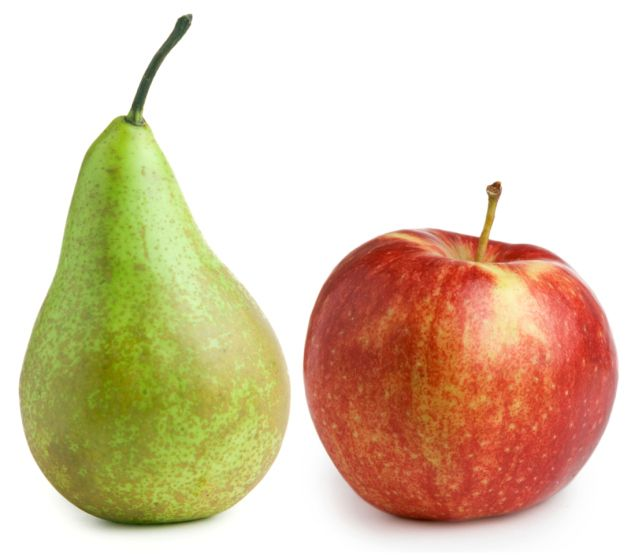
\includegraphics[width=0.25\textwidth]{markov/birneapfel}
    \caption{ Birne und Apfel unterscheiden sich durch Farbe, Form etc. - einen Stiel haben jedoch beide}
    \label{fig:apfelbirne}
\end{figure}


Die Extraktion signifikanter Merkmale ist ein wichtiger Teil von Machine Learning. Viele Eigenschaften eines Objektes sind nicht geeignet es von anderen zu unterscheiden. Im Apfel-Birnen-Beispiel würde das Merkmal ``Stiel'' nicht zu einer Unterscheidung führen.

Der nächste Schritt ist das Training des Systems. Hierbei wird zwischen drei algorithmischen Ansätzen unterschieden:
\begin{itemize}
\item Überwachtes Lernen
\item Unüberwachtes Lernen
\item Bestärkendes Lernen
\end{itemize}
Die häufigste menschliche Lernform, ist das bestärkende Lernen, hier wird mit ``Belohnung'' und ``Bestrafung'' gearbeitet. 
Im Machine Learning Bereich ist jedoch Überwachtes und Unüberwachtes Lernen sehr viel häufiger zu finden. Beim überwachten Lernen, werden mehrere Eingaben und Lösungen an den Algorithmus überreicht und nach einigen Durchgängen sollte er in der Lage  sein Assoziationen herzustellen. Je nach Algorithmus werden hierzu Funktionen und Gewichtungen angepasst. 

Das Hidden Markov Model ist im Bereich des Unüberwachten Lernens beheimatet. Aus der Menge der Eingaben wird ein Modell erzeugt, das Vorhersagen ermöglichen soll. Mit einem Expectation-Maximization-Algorithmus (EM-Algorithmus) wird versucht, die vorliegenden Daten in Kategorien einzuteilen, sodass die Daten optimal erklärt werden. Eine Form des EM-Algorithmus kommt auch beim Hidden Markov Model zum Einsatz.

Weitere Machine Learning Ansätze sind 
\begin{itemize}
\item Neuronale Netze
\item Support Vector Machine
\item K-Means
\end{itemize} 

\begin{figure}[htbp] \centering
    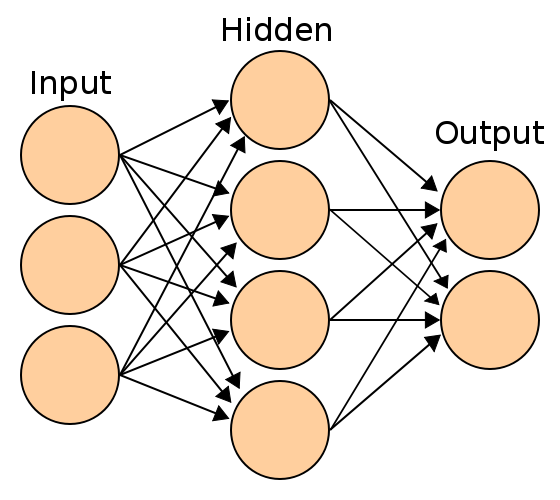
\includegraphics[width=0.4\textwidth]{markov/neuralnetwork}
    \caption{ Vereinfachte Darstellung eines neuronalen Netzwerkes mit 3 Merkmaldimensionen. }
    \label{fig:neural}
\end{figure}

Neuronale Netze versuchen das menschliche Gehirn mit seinen Neuronen und Synapsen nachzubauen \cite{neuron}. Für jede Dimension des Merkmalsvektors sind Neuronen vorhanden, welche wiederum mit anderen Neuronen verschaltet sind. Beim Training werden die Gewichtungen der einzelnen Verschaltungen verändert.
Abbildung \ref{fig:neural} \footnote{Quelle: \url{http://en.wikipedia.org/wiki/Artificial_neural_network\#/media/File:Artificial_neural_network.svg}} zeigt ein vereinfachtes neuronales Netz mit drei Inputs, vier weiteren Neuronen und zwei Outputs.

\begin{figure}[htbp] \centering
    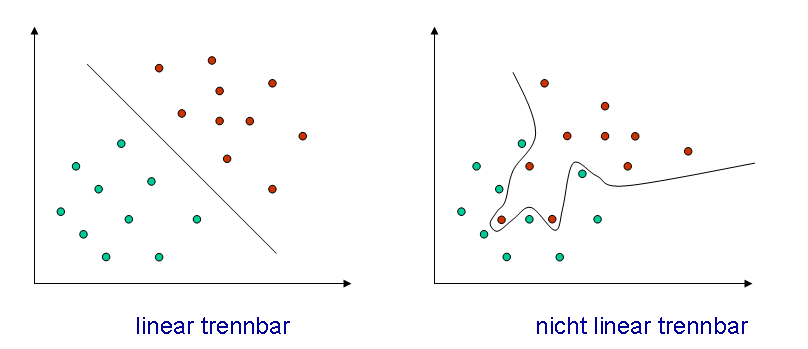
\includegraphics[width=0.5\textwidth]{markov/svm}
    \caption{ Daten lassen sich nicht immer linear trennen.}
    \label{fig:svm}
\end{figure}

Die Support Vector Machine (Stützvektormaschine) versucht die Daten durch lineare Trennung zu Klassifizieren (Siehe Abbildung \ref{fig:svm} \footnote{Quelle: \url{http://upload.wikimedia.org/wikipedia/de/a/a0/Diskriminanzfunktion.png}})
\cite{svm}. Es wird versucht, den Stützvektor möglichst weit von den beiden Klassen entfernt zu erstellen (Large-Margin-Classifier).


Im Abschnitt \ref{sec:compare} werden die vorgestellten Ansätze mit dem Hidden Markov Model verglichen.



\subsection{Wahrscheinlichkeitsrechnung}
Notwendige mathematische Grundlagen


  %%%%%%%%%%%%%%%%%%
  %  MARKOV-KETTE  % 
  %%%%%%%%%%%%%%%%%%  
\section{Markov Kette} 
\label{mainsec:mk}
Grundlage des Hidden Markov Model war die vom russischen Mathematiker Andrej Andrejewitsch Markov 
(1856 - 1922, siehe \cite{markov1913}) entwickelte Markov Kette. Zu Beginn des 20. Jahrhunderts beschäftigte er sich als erster mit einer statistischen Beschreibung von Zustands- und Symbolfolgen. Er führte eine statistische Analyse der Buchstabenfolge des Textes ``Eugene Onegin'' von Alexander 
Pushkin durch.

\subsection{Definition}
Eine Markov Kette beschreibt einen zeit-diskreten Prozess \((X_t)_{t\in\mathbb{N}_0}\) mit  \(m\) abzählbaren Zuständen \(S\) \cite{stochMod}.
Weiterhin wird sie als stationär bezeichnet, wenn alle Wahrscheinlichkeiten unabhängig von der Zeit sind.
Da die Verteilung der Zufallsvariablen nur von den vergangenen Zuständen abhängt, gilt eine Markov Kette als kausal \cite[48]{mmmFink}.
Wichtig für eine Markov Kette ist die sog. Markov-Eigenschaft:
\[ P (X_{t+1} = s_{t+1} | X_0 = s_0, \ldots , X_{t-1} = s_{t-1}, X_{t} = s_{t}) \]
\[ = P ( X_{t+1} = s_{t+1} | X_{t} = s_{t} ) \] \\
Genügt eine Markov Kette dieser Eigenschaft, wird sie als ``einfach'' oder Markov Kette 1. Ordnung bezeichnet.
Anders ausgedrückt beschreibt die Markov-Eigenschaft die Gedächtnislosigkeit des Prozesses, da der Folgezustand nur vom direkten Vorgänger abhängt.

Als Übergangswahrscheinlichkeit bezeichnte man die bedingte Wahrscheinlichkeit \(P ( X_{t+1} = s_{t+1} | X_{t} = s_{t} ) \), sodass auf 
den aktuellen Zustand \( s_{t}\) der Nachfolgezustand \( s_{t+1}\) folgt. Diese Wahrscheinlichkeiten werden üblicherweise zu einer Übergangsmatrix zusammengefasst: 
\[ A = [a_{ij}] =
\begin {bmatrix} 
  a_{00}&\cdots&a_{0m} \\
  \vdots&\ddots&\vdots \\
  a_{m0}&\cdots&a_{mm}
 \end {bmatrix} \forall i, j \in S \]
Da es sich um Wahrscheinlichkeiten handelt, muss sich die Summe jeder Reihe zu Eins addieren. \\

Weiterhin benötigt der Prozess einen Vektor für den Anfangzustand \( t = 0 \):
\[ \Pi = [ \pi_i] = [ P (X_0 = i) ] , i \in S \]

So lässt sich eine Markov-Kette durch Zustandsraum \(S\), den Übergangsmatrix \( A \) und einen Anfangszustand \( \Pi \) definieren.
Veranschaulichen lässt sich eine Markov Kette als gerichtetes Zustandsdiagramm (Abb. \ref{fig:simple_mc}) mit den Zuständen \(S\) und 
mit den Übergangswahrscheinlichkeiten \(X_i\) an den Kanten
\begin{figure}[htbp] \centering
    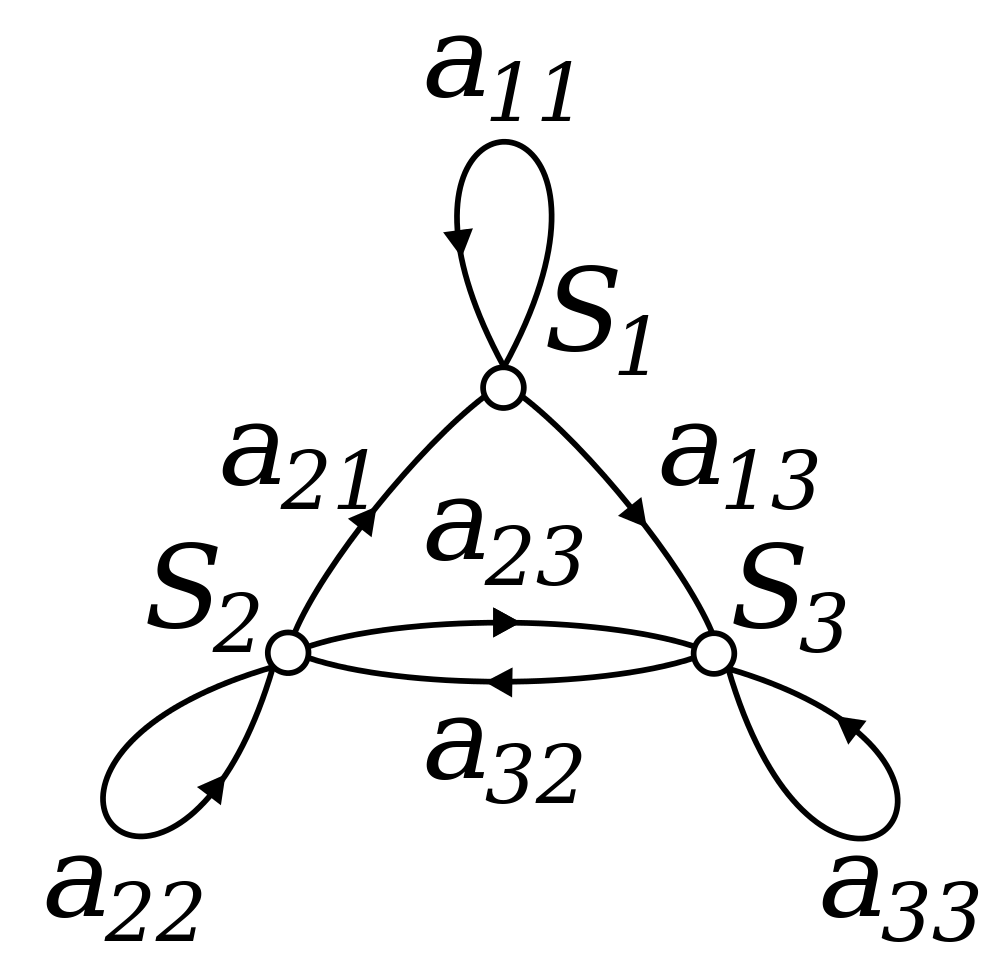
\includegraphics[width=0.5\textwidth]{markov/simple_mc.png}
    \caption{Einfaches Zustandsdiagramm einer Markov Kette (Quelle: \url{de.wikipedia.org/wiki/Markow-Kette})}
    \label{fig:simple_mc}
\end{figure}

Die Wahrscheinlichkeit für \( k \)-Schritte lässt sich so ausrechnen: 
\[ X_k = X_{k-1} A = X_0 A^k \] 


\subsection{Beispiel} 
\textit{ Markov Kette für das Wetter \footnote{Quelle: \url{en.wikipedia.org/wiki/Examples_of_Markov_chains}}} \\
Im folgenden Beispiel soll aufgrund des aktuellen Wetters auf das Wetter der folgenden Tage geschlossen werden.
Das Wetter kann entweder ``sunny'' oder ``rainy'' sein, zu Beginn (Tag 0, \( t = 0 \)) des Experiments ist es ``sunny''.
Die Wahrscheinlichkeit, dass auf ``sunny'' wieder ``sunny'' folgt, liegt bei 90\% (``rainy'' = 1 - ``sunny'' = 10\%). 
Nach ``rainy'' liegt die Wahrscheinlichkeit jeweils bei 50\% (siehe Abb. \ref{fig:simple_mc_example}).  
\begin{figure}[htbp] \centering
    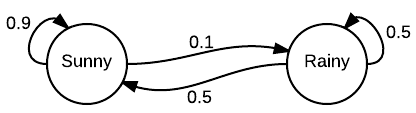
\includegraphics[width=0.5\textwidth]{markov/simple_mc_example.png}
    \caption{ Gerichteter Zustandsgraph der modellierten Wetter-Markov Kette }
    \label{fig:simple_mc_example}
\end{figure}


\[ Zust\ddot{a}nde: S = [``sunny'', ``rainy''] \]
\[ Anfangszustand:  \Pi = X_0 = [1 , 0] \]
\[\ddot{U}bergangsmatrix: A = \begin {bmatrix} 0.9&0.1\\0.5&0.5 \end {bmatrix}
\]

Nun kann die Wahrscheinlichkeit für das Wetter an Tag 1 berechnet werden über: \\
\[ X_1 = X_0 * A = [ 1, 0 ] \begin {bmatrix} 0.9&0.1\\0.5&0.5 \end {bmatrix} = [ 0.9, 0.1] \]

Für Tag 2:\\
\[ X_2 = X_1 A = X_0 A^2 = [ 1, 0 ] \begin {bmatrix} 0.9&0.1\\0.5&0.5 \end {bmatrix}^2 = [ 0.86, 0.14] \] 

Verallgemeinert für Tag k bedeutet das: 
\[ X_k = X_{k-1} A = X_0 A^k = [ 1, 0 ] \begin {bmatrix} 0.9&0.1\\0.5&0.5 \end {bmatrix}^k \] 

  %%%%%%%%%%%%%%%%%%
  %  HIDDEN-MARKOV  % 
  %%%%%%%%%%%%%%%%%%
\section{Hidden Markov Model}
\label{mainsec:hmm}

Das Hidden Markov Model ist ein stochastisches Modell für sequentielle Daten und wird vor allem in der Spracherkennung und in der Bioinformatik eingesetzt. 
Der amerikanischen Mathematiker Leonard E. Baum (* 1931) und andere Autoren entwickelten auf Basis der Markov Kette Ende der 
sechziger Jahre das Hidden Markov Model \cite{baum66}. Erste Hidden Markov Model-Applikationen wurden zur Spracherkennung und später auch in der Bioinformatik zur Analyse von Nukleotid- und Proteinsequenzen eingesetzt. 


\subsection{Definition}
Ein Hidden Markov Model erweitert eine Markov Kette um eine weiteren Zufallsprozess und ist somit ein zweistufiger stochastischer Prozess \cite[67]{mmmFink}. Hierfür wird
jedem Zustand der Markov Kette eine Ausgabe bzw. Emission zugeordnet dessen Wahrscheinlichkeitsverteilung einzig vom aktuellen Zustand abhängig ist. Die Emissionen sind die einzigen beobachtbaren Zustände des Hidden Markov Model. Der Rest ist sozusagen 'versteckt' woher sich auch der Name des Models ableitet. Eine Folge von Emissionen wird auch Observationsfolge genannt.


Das Hidden Markov Model wird definiert durch \cite[68]{mmmFink}:\\ 
\( \lambda = (S;V;A;B;\pi)\)
\begin{itemize}
     \item Endlich Menge von Zuständen \\
           \( S = \{ s | 1 <= s <= N \} \)
     \item Alphabeth der Emissionen \\
           \( V = \{ v | 1 <= v <= M \} \)
     \item Matrix der Zustandsübergangs-wahrscheinlichkeiten \\
           \( A = \{ a_{ij} | a_{ij} = P(S_t = j | S_{t-1} = i) \} \)
     \item Matrix der Emissionsverteilung \\
           \( B = \{ b_{jk} | b_{jk} = P(O_t = o_k | S_t = j) \} \) bzw. \( B =
           \{ b_{j}(x) | b_{j}(x) = p(x|S_t = j) \} \)
     \item Vektor von Zustandsstartwahrscheinlichkeiten \\
           \( \pi = \{ \pi_i | \pi_i = P(S_1 = i) \} \) 
\end{itemize}

Die Emissionsmodellierung ist hierbei vom Kontext der Problemstellung abhängig. Wird das Hidden Markov Model zum Beispiel bei der Analyse von biologischen Sequenzen, sprich einem diskreten Symbolinventar, angewendet, wird ein diskretes  Emissionsmodel genutzt. Man spricht hierbei auch von einem diskreten Hidden Markov Model. Wenn dieses Model zur verarbeitung von Signalen verwendet werden soll erfordert dies in der Vorverarbeitung der Daten einen Quantisierer der die  kontinuerlichen Merkmale in eine diskrete Observationsfolge überführt. 

Gängiger ist es hierfür kontinuierliche Hidden Markov Model's zu nutzen. Hierbei wird eine Emissionsmodelierung auf Basis kontinuierlicher Dichtefunktionen genutzt die kontinuierliche Observationen im \(\mathbb{R}^n\) verarbeitet.\\ 
\( B =\{ b_{j}(x) | b_{j}(x) = p(x|S_t = j) \} \)\\
Zur behandlung kontinuerlicher Verteilungen mit mehreren komplexen Häufigkeitsgebieten werden approximatische Verfahren genutzt. Die verbreiteste Technik besteht aus der Verwendung von Mischverteilungen auf der Basis von Gauß-Dichten (Gaussian Mixture Model). Man kann nämlich zeigen, dass sich jede allgemeine kontinuierliche Verteilung \(p(x)\) durch eine Linearkombination von i.a. unendlich vielen Basis-Normalverteilungen beliebig genau approximieren lässt\cite[69]{mmmFink}:
 
\begin{multline}
p(x) \hat{=} \sum_{k=1}^\infty c_{k} N(x|\mu_{k},K_{k})\\
\approx \sum_{k=1}^M c_{k} N(x|\mu_{k},K_{k})  
\end{multline}
Der Approximationsgfehler lässt sich hierbei über eine geeignete Anzahl von \(M\) Basisverteilungen klein halten. Somit ergibt sich für die Beschreibung der Emissionsverteilung eines Zustands des Hidden Markov Model folgende Formel:
\begin{equation}
b_{j}(x) = \sum_{k=1}^M c_{jk}g_{jk}(x)
\end{equation}
Die Anzahl der Basisverteilungen eines Gaussian Mixture Model kann hierbei für die einzelnen Zustände des HMM variieren.\\


\subsection{Beispiel}
\begin{figure}[htbp] \centering
    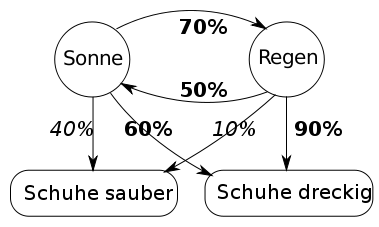
\includegraphics[width=0.4\textwidth]{markov/hmm_example.png}
    \caption{Hidden Markov Model für das Beipiel des Gefangen im Verlies}
    \label{fig:hmm_example}
\end{figure}

Abbildung \ref{fig:hmm_example} soll ein Hidden Markov Model an dem Beispiel des Gefangenen im Verlies  darstellen\footnote{Quelle: \url{http://de.wikipedia.org/wiki/Hidden_Markov_Model}}. Ein Gefangener im Kerkerverlies möchte das aktuelle Wetter herausfinden. Er weiß, dass auf einen sonnigen Tag zu 70 \% ein Regentag folgt und dass auf einen Regentag zu 50 \% ein Sonnentag folgt. Weiß er zusätzlich, dass die Schuhe der Wärter bei Regen zu 90 \% dreckig, bei sonnigem Wetter aber nur zu 60 \% dreckig sind, so kann er durch Beobachtung der Wärterschuhe Rückschlüsse über das Wetter ziehen (das heißt, er kann die Wahrscheinlichkeit für Regenwetter gegenüber sonnigem Wetter abschätzen). Sonne und Regen sind in diesem Fall die versteckten Zustände. Die  Emissionen bzw. die Observation die der Gefangene machen kann sind nur der Verschmutzungsgrad der Schuhe der Wärter.


\subsection{Funktionsweise}
Das Konzept des Hidden Markov Model kann laut \cite{rabiner} in drei Problemstellungen eingeteilt werden:
\begin{itemize}
  \item Evaluierungsproblem: Bestimme die Wahrscheinlichkeit für ein Model mit
  der dieses eine gegebene Observationsfolge erzeugt.
  \item Dekodierungsprobem: Finde interne Abläufe für eine gegebene Observationsfolge
  \item Trainingsproblem: Finde Modellparameter für gegebene Beispieldaten
\end{itemize}

\textbf{Evaluierung} \\
In der Evaluierung soll die Wahrscheinlichkeit bestimmt werden mit der eine
betrachtete Observationsfolge in einer beliebigen Zustandsfolge von einem
gegebenen Hidden Markov Model \(\lambda\) generiert wird. Diese Wahrscheinlichkeit wird
Produktionswahrscheinlichkeit genannt. Diese wird mit dem Forward-Algorithmus
berechnet. Der Algorithmus nutzt hierfür die geltende Markov Eigenschaft
aus das nur die Speicherung eines internen Zustandes erlaubt. Hierfür definiert
man als Vorwärtsvariable \(\alpha_{t}(i)\) die Wahrscheinlichkeit, bei
gegebenem Model $\lambda$ den Anfang der betrachteten Observationsfolge \(O_{t}\)
zu erzeugen und zum Zeitpunkt \(t\) den Zustand i zu erreichen.
\begin{equation}
\alpha_{t}(i) = P(O_{1},O_{2},\ldots,O_{t},s_{t}=i|\lambda)
\end{equation}
Die Vorwährtsvariable lässt sich nun mit den folgenden Schritten rekursiv
berechnen um die Gesamtwahrscheinlichkeit des Models zu erhalten.
\begin{enumerate}
  \item Initialisierung\\
		$\alpha_{1}(i) := \pi_{i}b{i}(O_{1})$
  \item Rekursion\\
	für alle Zeitpunkte \(t, t=1 \ldots T-1\)\\
	\(\alpha_{t+1}(j) :=
	\sum\limits_{i}\{\alpha_{t}(i)\alpha_{ij}\}b_{j}(O_{t+1})\)
  \item Rekursionsabschluss\\
  	\(P(O|\lambda) = \sum\limits_{i=1}^N \alpha_{T}(i)\)
\end{enumerate}


\textbf{Dekodierung} \\
Bei der Dekodierung soll die optimale, bzw. wahrscheinlichste Zustandsfolge
\(s^*\) aus der Menge der Zustände ermittelt werden die eine gegebene
Observationsfolge erzeugt. Zur Ermittlung der optimalen Zustandsfolge bedient
man sich des Viterbi-Algorithmus, einem induktiven Verfahren das dem Forward
Algorithmus sehr ähnlich ist. Zu Begin werden erneut die Wahrscheinlichkeiten
\(\delta_{t}(i)\) für partiell optimale Pfade definiert, die das Anfangssegment
der Observationsfolge bis \(O_{t}\) mit maximaler Wahrscheinlichkeit erzeugen
und in Zustand \(i\) enden.
\begin{equation}
\delta_{t}(i) =
\max\limits_{s_{1},s_{2}, \ldots
,s_{t}}P(O_{1},\ldots,O_{t},s_{1},\ldots,s_{t}=i|\lambda) 
\end{equation}
Der Algorithmus entspricht weitgehend dem Forward-Algorithmus jedoch werden
anstatt der Summe im Rekursionsabschluss, die Maximalen über die in den
Vorgängerzuständen vorliegenden Wahrscheinlichkeiten gebildet.
\begin{enumerate}
  \item Initialisierung\\
		\(\delta_{1}(i) := \pi_{i}b{i}(O_{1})\)\\
		\(\phi_{1}(i):=0\)
  \item Rekursion\\
	für alle Zeitpunkte \(t, t=1 \ldots T-1\)\\
	\(\delta_{t+1}(j) :=
	\max\limits_{i}\{\delta_{t}(i)\alpha_{ij}\}b_{j}(O_{t+1})\)\\
	\(\phi_{t+1}(j):= \operatorname{arg\,max}\limits_{i}\{\lambda_{t}(i)\alpha_{ij} \)
  \item Rekursionsabschluss\\
  	\(P^{*}(O|\lambda) = (P(O,s^{*}|\lambda) = \max_{i}\lambda_{T}(i)
  	\alpha_{T}(i)\)
  \item Rückverfolgung des Pfades\\
	für alle Zeitpunkte \(t, t=1 \ldots T-1\)\\
	\(s_{t}^{*}=\phi_{t+1}(s_{t+1}^{*})\)
\end{enumerate}
Mit \(\phi_{t}(j)\) wird ein ``Rückwärtszeiger'' definiert der für jedes
entsprechende \(\delta_{t}(j)\) entlang der partiellen Pfade den jeweils
optimalen Vorgängerzustand speichert.\\

\textbf{Training} \\
Je nach Problemstellung müssen unterschiedliche Modelle eines HMM's gewählt
werden. Es ist bisher kein Verfahren bekannt das aufgrund einer Stichprobe ein
Optimales Modell generieren kann. Die Anzahl der Zustände, die Wahl der
Emissionsverteilungen sowie deren initialer Parameterwerte müssen nach eigenen Erfahrungen gewählt werden. Wenn dies geschehen ist kann das Modell in einem iterativen Prozess trainiert werden. Hierbei werden die Parameter einer Wachstumstransformation unterworfen. Ziel ist es das die Modellparameter so verändert werden das die Bewertung des veränderten Models besser als die des Ausgangsmodels ist.\\

Zum trainieren eines Hidden Markov Model existieren diverse Algorithmen. Sie unterscheiden sich im wesentlichen durch die Verwendeten Qualitätsmaße zur Bewertung der Modelierungsgüte. Beim Baum-Welch-Algorithmus \cite{rabiner} wird die Produktionswahrscheinlichkeit \(P(O|\lambda)\) zur Bewertung genutzt. Beim Viterbi-Algorithmus \cite{viterbi} und dem eng verwandten Segmental-k-means Algorithmus \cite{juang} nur die Wahrscheinlichkeit \((P(O,s^{*}|\lambda)\) der jeweils optimalen Zustandsfolge betrachtet \cite{mmmFink}.



  %%%%%%%%%%%%
  %  RESULT  % 
  %%%%%%%%%%%%
\section{Zusammenfassung}  \label{mainsec:result}

\subsection{Fazit}
Wie schlägt sich ein HMM in der Praxis

\subsection{Vergleich mit anderen Machine Learning Ansätzen}
\label{sec:compare}
Wie arbeiten Neuronale Netze, SVM, k-Means und Co. im Vergleich?


% Can use something like this to put references on a page
% by themselves when using endfloat and the captionsoff option.
\ifCLASSOPTIONcaptionsoff
  \newpage
\fi



% trigger a \newpage just before the given reference
% number - used to balance the columns on the last page
% adjust value as needed - may need to be readjusted if
% the document is modified later
%\IEEEtriggeratref{8}
% The "triggered" command can be changed if desired:
%\IEEEtriggercmd{\enlargethispage{-5in}}

% references section

% can use a bibliography generated by BibTeX as a .bbl file
% BibTeX documentation can be easily obtained at:
% http://www.ctan.org/tex-archive/biblio/bibtex/contrib/doc/
% The IEEEtran BibTeX style support page is at:
% http://www.michaelshell.org/tex/ieeetran/bibtex/
%\bibliographystyle{IEEEtran}
% argument is your BibTeX string definitions and bibliography database(s)
%\bibliography{IEEEabrv,../bib/paper}
%
% <OR> manually copy in the resultant .bbl file
% set second argument of \begin to the number of references
% (used to reserve space for the reference number labels box)
\begin{thebibliography}{1}

% http://www.cs.uni-potsdam.de/ml/teaching/ss10/st/HMMs.pdf

\bibitem[Mar09]{marsland}
Stephen Marsland.
\newblock {\em Machine Learning - An Algorithmic Perspective.}
\newblock Chapman I\& Hall, 2009.


\bibitem[McC43]{neuron}
W. McCulloch und W. Pitts
\newblock{\em A logical calculus of the ideas immanent in nervous activity.}
\newblock Bulletin of Mathematical Biophysics, 5:115-133, 1943,

\bibitem[BGV92]{svm}
Boser, B. E.; Guyon, I. M.; Vapnik, V. N.
\newblock{ \em A training algorithm for optimal margin classifiers.}
\newblock Proceedings of the fifth annual workshop on Computational learning theory - COLT '92. p. 144. 1992

\bibitem[Mar13]{markov1913}
A.A. Markov.
\newblock {\em Example of a statistical investigation of the text of ``Eugene Onegin'' illustrating the dependence between samples in chain}.
\newblock translated by alexander y. nitussov, lioudmila voropai and david link, 1913.

\bibitem[Bau66]{baum66}
Baum, L. E. and Petrie, T. 
\newblock {\em Statistical Inference for Probabilistic Functions of Finite State Markov Chains}. 
\newblock The Annals of Mathematical Statistics 37 (6): 1554–1563. 1966

\bibitem[Rab89]{rabiner}
Lawrence~R. Rabiner.
\newblock {\em A tutorial on hidden markov models and selected applications in speech recognition.}
\newblock In {\em Proceedings of the IEEE}, pages 257--286, 1989.

\bibitem[Han08]{handel}
R.v. Handel 
\newblock{\em Hidden Markov Models} 
\newblock{ Lecture Notes Princeton University, 2008. }

\bibitem[KHW13]{stochMod}
U.M.~Stocker K.-H.~Waldmann.
\newblock {\em Stochastische Modelle - Eine anwendungsorientierte Einführung}.
\newblock Springer-Verlag, Berlin Heidelberg, 2013.

\bibitem[Fin03]{mmmFink}
Gernot~A. Fink.
\newblock {\em Mustererkennung mit Markov-Modellen}.
\newblock B. G. Teubner Verlag, 2003.

\bibitem[Vit67]{viterbi}
A. Viterbi
\newblock {\em Error Bounds for Convolutional Codes and an Asymptotically Optimum Decoding Algorithm}.
\newblock IEEE Trans. Inf. Theor, 1967.


\bibitem[Jua90]{juang}
Juang, B. H. and Rabiner, L. R.
\newblock {\em The segmental K-means algorithm for estimating parameters of hidden Markov models}.
\newblock Acoustics, Speech and Signal Processing, IEEE Transactions on 1990.

\end{thebibliography}

\end{document}


